\documentclass[12pt]{article}

\usepackage[margin=1in]{geometry}
\usepackage{enumitem}
\usepackage{listings}
\usepackage{xcolor}
\usepackage{hyperref}
\usepackage{graphicx}
\usepackage{parskip}

\lstset{
  language=C,
  basicstyle=\ttfamily\small,
  keywordstyle=\color{blue},
  commentstyle=\color{gray},
  stringstyle=\color{red},
  breaklines=true,
  frame=single,
  numbers=none,
  xleftmargin=1em,
  framexleftmargin=1em,
}

\title{CSC209: Systems Programming Mini-Project}
\author{Elvis Chen \and Prabeer Sohal \and Rian Mehta}
\date{}

\begin{document}

\maketitle

%% ─────────────────────────────────────────────
\section{Project Overview}
%% ─────────────────────────────────────────────

This project is a multi-process application using pipes (Category~1). The
program performs sentiment analysis on input text by distributing sentences
across multiple worker processes and collecting their results.

The parent process reads text from standard input, splits the input into
sentences based on punctuation, and assigns each sentence to a worker
process. Each worker computes a sentiment score and sends the result back
to the parent through a pipe. In \texttt{main.c}, the parent process
creates five worker processes using \texttt{fork()} (line~106) and
establishes two pipes per worker for communication. Each worker executes
the \texttt{worker()} function (\texttt{main.c}:41), where it waits for
input, processes a sentence using \texttt{predict()} from
\texttt{model.c}, and returns a result. Communication is done using
fixed-size messages defined by the \texttt{SentenceMsg} and
\texttt{Result} structures (\texttt{main.c}:16--25), which ensures
consistent and predictable data transfer between processes.

The program accepts input through standard input. Users can type input
interactively or pipe text from another command or file, for example:

\begin{lstlisting}[language=bash]
echo "This is good. This is bad." | ./sentiment -a
\end{lstlisting}

In default mode, the program outputs summary statistics such as the total
number of sentences analyzed, the number of positive and negative
sentences, the average sentiment score, and the overall sentiment. When
the \texttt{-a} flag is used, the program prints detailed results for each
sentence, including the sentence text, its predicted label, and its score.

The main concepts of the project are process creation, concurrency, and
inter-process communication using pipes. The sentiment model serves as the
computational task assigned to each worker, while the parent process
coordinates task distribution and result collection.

%% ─────────────────────────────────────────────
\section{Build Instructions}
%% ─────────────────────────────────────────────

The project can be compiled using the provided \texttt{Makefile}. To build
the project, run:

\begin{lstlisting}[language=bash]
make
\end{lstlisting}

This compiles all \texttt{.c} files with the flags \texttt{-Wall -Wextra
-g} and produces two executables:

\begin{itemize}
  \item \texttt{sentiment} --- the main program.
  \item \texttt{test} --- a helper program used to test sentiment
        prediction on a single sentence.
\end{itemize}

The \texttt{Makefile} ensures that all object files are built first and
then linked together. It also links the math library using \texttt{-lm},
which is required for functions such as \texttt{expf()} used in
\texttt{model.c}.

To run the main program:

\begin{lstlisting}[language=bash]
./sentiment
\end{lstlisting}

The program reads input from standard input. Users can type input manually
and press \texttt{Ctrl+D} to signal the end of input, or provide input
using a pipe or file redirection:

\begin{lstlisting}[language=bash]
echo "This is good. This is bad." | ./sentiment -a
\end{lstlisting}

To display detailed results for each sentence, use the \texttt{-a} flag:

\begin{lstlisting}[language=bash]
./sentiment -a
\end{lstlisting}

The \texttt{test} program can be used to evaluate a single sentence:

\begin{lstlisting}[language=bash]
./test "this is great"
\end{lstlisting}

To remove all compiled files, including object files and executables:

\begin{lstlisting}[language=bash]
make clean
\end{lstlisting}

The program requires the files \texttt{weights.bin} and
\texttt{vocab.bin} to be present in the working directory. If these files
are missing, the program will print an error and exit
(\texttt{main.c}:83--90).

%% ─────────────────────────────────────────────
\newpage
\section{Architecture Diagram}
%% ─────────────────────────────────────────────

\begin{figure}[h]
  \centering
  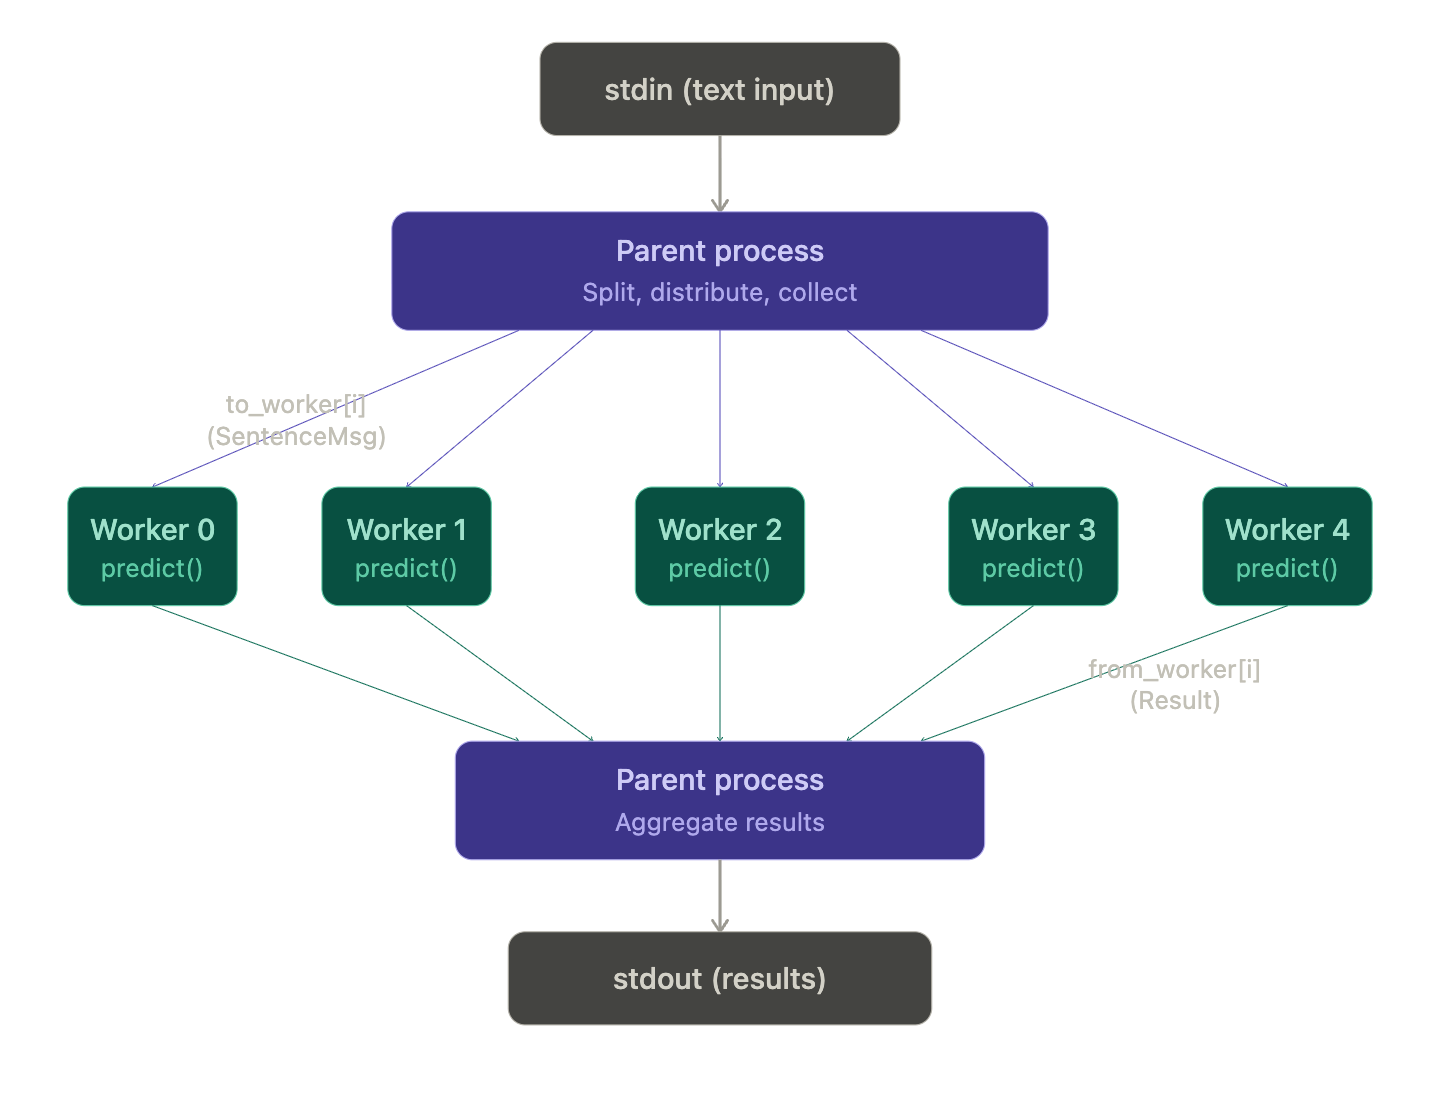
\includegraphics[width=0.85\textwidth]{diagram.png}
  \caption{Architecture of the multi-process sentiment analysis pipeline.}
  \label{fig:arch}
\end{figure}

%% ─────────────────────────────────────────────
\newpage
\section{Communication Protocol}
%% ─────────────────────────────────────────────

The program uses pipes for communication between the parent and worker
processes. Each worker has two dedicated pipes: one for receiving tasks
from the parent and one for sending results back. Communication is
implemented using fixed-size binary messages, which simplifies parsing and
ensures consistent message boundaries. Two message types are used:
\texttt{SentenceMsg} and \texttt{Result}.

%% ── SentenceMsg ──────────────────────────────
\subsection{Message Type: SentenceMsg}

\begin{description}[style=nextline]
  \item[Sender] Parent
  \item[Receiver] Worker
  \item[Encoding]~

\begin{lstlisting}
typedef struct {
    uint32_t job_id;
    uint32_t len;
    char     text[MAX_SENTENCE]; // MAX_SENTENCE = 1024
} SentenceMsg;
\end{lstlisting}

  \item[Semantics]
    This message represents a task assigned to a worker. The parent
    constructs a \texttt{SentenceMsg} in \texttt{main.c} (lines~206--209)
    after extracting a sentence from the input. The \texttt{job\_id}
    uniquely identifies the sentence, allowing the parent to match results
    to their original order. The \texttt{len} field indicates the length of
    the sentence, and \texttt{text} contains the null-terminated sentence
    itself.

  \item[Invariants]~
    \begin{itemize}
      \item The worker reads exactly \texttt{sizeof(SentenceMsg)} bytes
            using \texttt{read\_full()} (\texttt{main.c}:27--39).
      \item Each \texttt{job\_id} is unique and assigned sequentially.
      \item The \texttt{text} field is null-terminated.
      \item The value of \texttt{len} matches the actual sentence length.
    \end{itemize}

  \item[Error handling]
    The worker validates incoming messages when reading from the pipe. In
    the \texttt{worker()} function (\texttt{main.c}:41), \texttt{read\_full()}
    is used to ensure that a complete \texttt{SentenceMsg} is received. If
    \texttt{read\_full()} returns~0, it indicates that the pipe has been
    closed, and the worker exits. If it returns a negative value, it
    indicates a read error, and the worker also terminates.

    The \texttt{len} field is used to detect termination. A message with
    \texttt{len == 0} is interpreted as a shutdown signal, sent by the
    parent after all jobs have been processed (\texttt{main.c}:236--242).
    This ensures that workers exit cleanly without requiring external
    signals.

    Since each pipe has a single writer, there is no risk of interleaved
    messages. The use of \texttt{read\_full()} further guarantees that the
    worker does not process incomplete data.
\end{description}

%% ── Result ───────────────────────────────────
\subsection{Message Type: Result}

\begin{description}[style=nextline]
  \item[Sender] Worker
  \item[Receiver] Parent
  \item[Encoding]~

\begin{lstlisting}
typedef struct {
    uint32_t job_id;
    float    score;
} Result;
\end{lstlisting}

  \item[Semantics]
    This message contains the result of processing a sentence. The worker
    computes the sentiment score in the \texttt{worker()} function
    (\texttt{main.c}:41) using \texttt{predict()} from \texttt{model.c}
    (line~23). The \texttt{job\_id} is copied from the original
    \texttt{SentenceMsg} so the parent can store the result in the correct
    position.

  \item[Invariants]~
    \begin{itemize}
      \item The parent reads exactly \texttt{sizeof(Result)} bytes using
            \texttt{read\_full()}.
      \item The \texttt{job\_id} corresponds to a previously sent task.
      \item The \texttt{score} is a floating-point value between 0 and~1.
    \end{itemize}

  \item[Error handling]
    The program uses \texttt{read\_full()} (\texttt{main.c}:27--39) to
    read data from pipes. This function repeatedly calls \texttt{read()}
    until the requested number of bytes has been received or an error
    occurs, preventing issues caused by partial reads.

    Write operations are checked for errors in both the parent and worker
    processes. If a write fails, an error message is printed using
    \texttt{perror()}, and the process exits or stops using the pipe
    (\texttt{main.c}:57--60, 211--214).
\end{description}

%% ─────────────────────────────────────────────
\section{Concurrency Model}
%% ─────────────────────────────────────────────

The program achieves concurrency by creating five worker processes using
\texttt{fork()} in \texttt{main.c} (lines~105--132) after all pipes are
initialized. The parent forks all workers before distributing any tasks;
each worker immediately begins executing the \texttt{worker()} function
(\texttt{main.c}:41) and blocks on \texttt{read\_full()} waiting for
input. This blocking behavior means workers are always ready to receive
tasks without requiring explicit readiness checks.

The parent distributes sentences in a round-robin manner across workers by
writing \texttt{SentenceMsg} structures to their input pipes
(\texttt{main.c}:211). To avoid deadlock, the parent tracks the number of
active jobs using the \texttt{active\_jobs} variable
(\texttt{main.c}:161). The parent sends tasks freely until all five
workers are busy (\texttt{active\_jobs == NUM\_WORKERS}), at which point
it blocks to collect one result from the oldest outstanding worker before
sending the next task (\texttt{main.c}:184--194).

Results are collected through blocking reads from worker output pipes and
stored using \texttt{job\_id} to preserve the original sentence ordering
(\texttt{main.c}:186--188). After all tasks have been dispatched and all
results collected (\texttt{main.c}:223--233), the parent sends a
zero-length termination message to each worker
(\texttt{main.c}:236--242) and uses \texttt{waitpid()} to collect all
child processes (\texttt{main.c}:247--250), ensuring no zombie processes
remain.

%% ─────────────────────────────────────────────
\section{Error Handling and Robustness}
%% ─────────────────────────────────────────────

\begin{enumerate}[label=(\roman*)]

  \item \textbf{Worker reads from a closed pipe or encounters end of
  file.}
  In the \texttt{worker()} function (\texttt{main.c}:41), each worker
  calls \texttt{read\_full()} to receive a \texttt{SentenceMsg}. If
  \texttt{read\_full()} returns~0 (end of file) or a negative value
  (error), the worker exits the loop and terminates cleanly by closing
  its file descriptors and calling \texttt{exit(0)}
  (\texttt{main.c}:63--65). This prevents the worker from processing
  invalid or incomplete data.

  \item \textbf{Write to a closed pipe.}
  If a worker or the parent attempts to write to a pipe whose read end
  has been closed, the \texttt{write()} call will fail. In both
  \texttt{main.c}:57 (worker side) and \texttt{main.c}:211 (parent
  side), all \texttt{write()} calls check the return value. Failures are
  reported using \texttt{perror()}, and the process stops using the pipe
  to avoid undefined behavior.

  \item \textbf{Memory allocation failure.}
  The program dynamically allocates memory for buffers and arrays using
  \texttt{malloc()} and \texttt{realloc()}. All allocation calls are
  checked for \texttt{NULL} (e.g., \texttt{main.c}:139, 146, 156). If
  an allocation fails, an error message is printed and the program exits,
  preventing dereferencing of invalid pointers.

  \item \textbf{Malformed or unexpected input.}
  Input is read and split into sentences in \texttt{main.c}
  (lines~165--218). Empty sentences are skipped (line~176), and sentences
  longer than \texttt{MAX\_SENTENCE} are truncated (line~177) before
  being copied into a \texttt{SentenceMsg}. This ensures that messages
  always fit within the fixed-size buffer and prevents buffer overflows.

\end{enumerate}

%% ─────────────────────────────────────────────
\section{Team Contributions}
%% ─────────────────────────────────────────────

\textbf{Elvis Chen.}

I am in charge of training the model in python, which is available at \url{github.com/pythomiere/SAM} and implement the model in C.
% Describe Elvis's specific contributions here.

\medskip
\textbf{Prabeer Sohal.}

I am in charge of the \texttt{Makefile} and writing the report. 
% Describe Prabeer's specific contributions here.

\medskip
\textbf{Rian Mehta.}

I am in charge of writing \texttt{main.c} and making the demo video.
% Describe Rian's specific contributions here.

\end{document}
